\chapter{Ergebnisanalyse} \label{chap:ergebnisanalyse}
Wie der Output einer Error-Level-Analyse haben uns die vorherigen Programmtests schon gezeigt. In diesem Kapitel wird aufgezeigt welche Informationen sich aus dem Ergebnisbild gewinnen lassen. Nicht alle besonders hellen Bereiche des ELA-Bildes sind ein Beweis für eine Fotomontage. Es ist wichtig hier das Gesamtbild zu betrachten.

\section{Mehrfachkompression} \label{chap:mehrfachkompression}
Die Menge der Fehler, welche durch eine erneute Komprimierung in einem Bild herbeigeführt werden sind nicht linear. So ist das Bild, welches man in der Qualitätsstufe 75\% speichert und anschließend erneut mit 90\% speichert, fast identisch mit dem Bild welches man von 90\% nach 75\% erzeugt oder fast identisch mit dem Bild welches man einmalig bei 67,5\% speichert.\cite{Krawetz2008}\\
Umso heller die Bereiche in einem generierten ELA-Bild sind, desto mehr Veränderungen sind durch die Rekompression entstanden. Dahingegen gilt, dass je dunkler ein Bereich ist, desto weniger oder keine Veränderungen hat es bei der erneuten Kompression gegeben. Nach etwa 64 Speichervorgängen gibt es praktisch keine Veränderung mehr.\\
Die folgenden Abbildungen sollen darstellen wie sich das erzeugte ELA-Bild gegenüber erneuten abspeichern verhält. Dabei wurden alle Bilder mit der selben Software und den selben Parametern erstellt. Für die JPEG-Qualität wurden 88\% vorgegeben und für die Fehlertoleranz 30\%.
\autoref{fig:elaOriginal} zeig das Bild im Originalzustand und dessen Error-Level-Analyse. \autoref{fig:elaPhotoshop} zeigt das Bild nach einmaligem abspeichern in Adobe Photoshop mit der Qualitätseinstellung 70\%. Der Vergleich beider Bilder zeigt deutlich, dass das Bild nach der erneuten Kompression weniger helle stellen aufweist als das Originale. Würde man das Bild noch mehrmals in Adobe Photoshop neu laden und wieder mit der selben Qualitätseinstellung abspeichern würde es mit jedem male ein wenig dunkler werden. Der Effekt ist nach der ersten Komprimierung allerdings nur noch marginal sichtbar. 

\begin{figure}[H]
	\begin{center}
		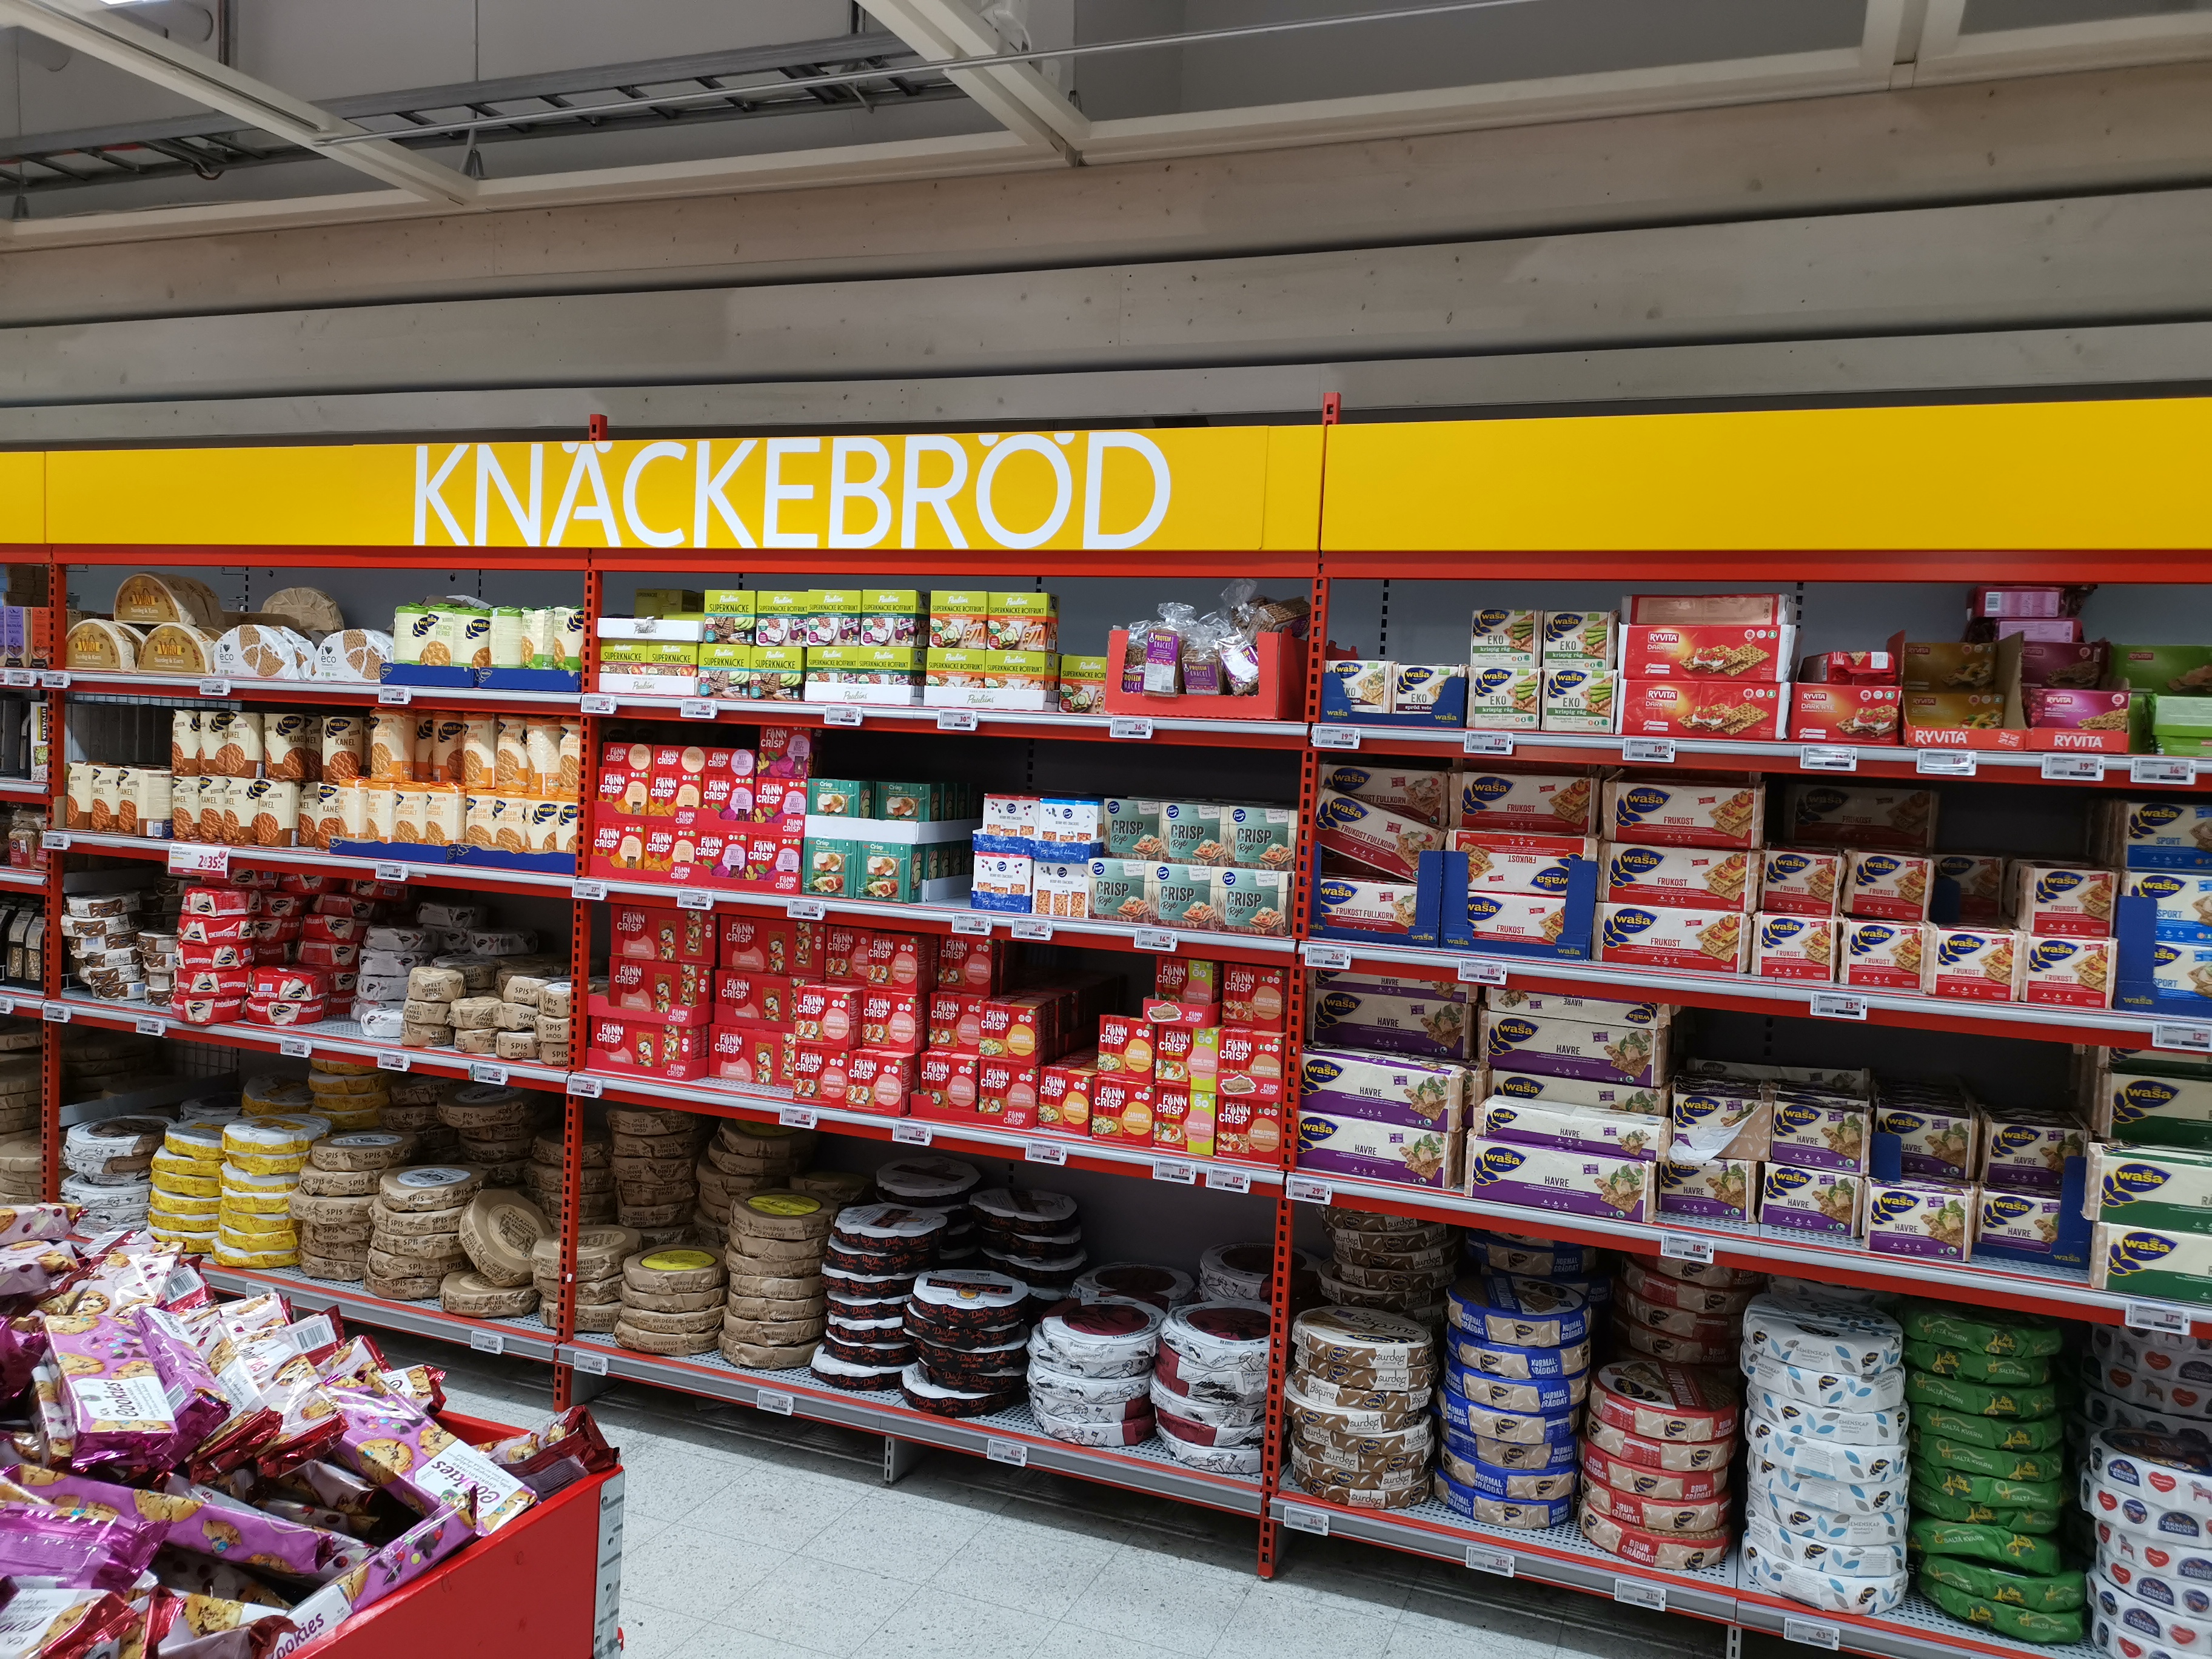
\includegraphics[width=0.4\linewidth]{images/knackebrot/original.jpg}
		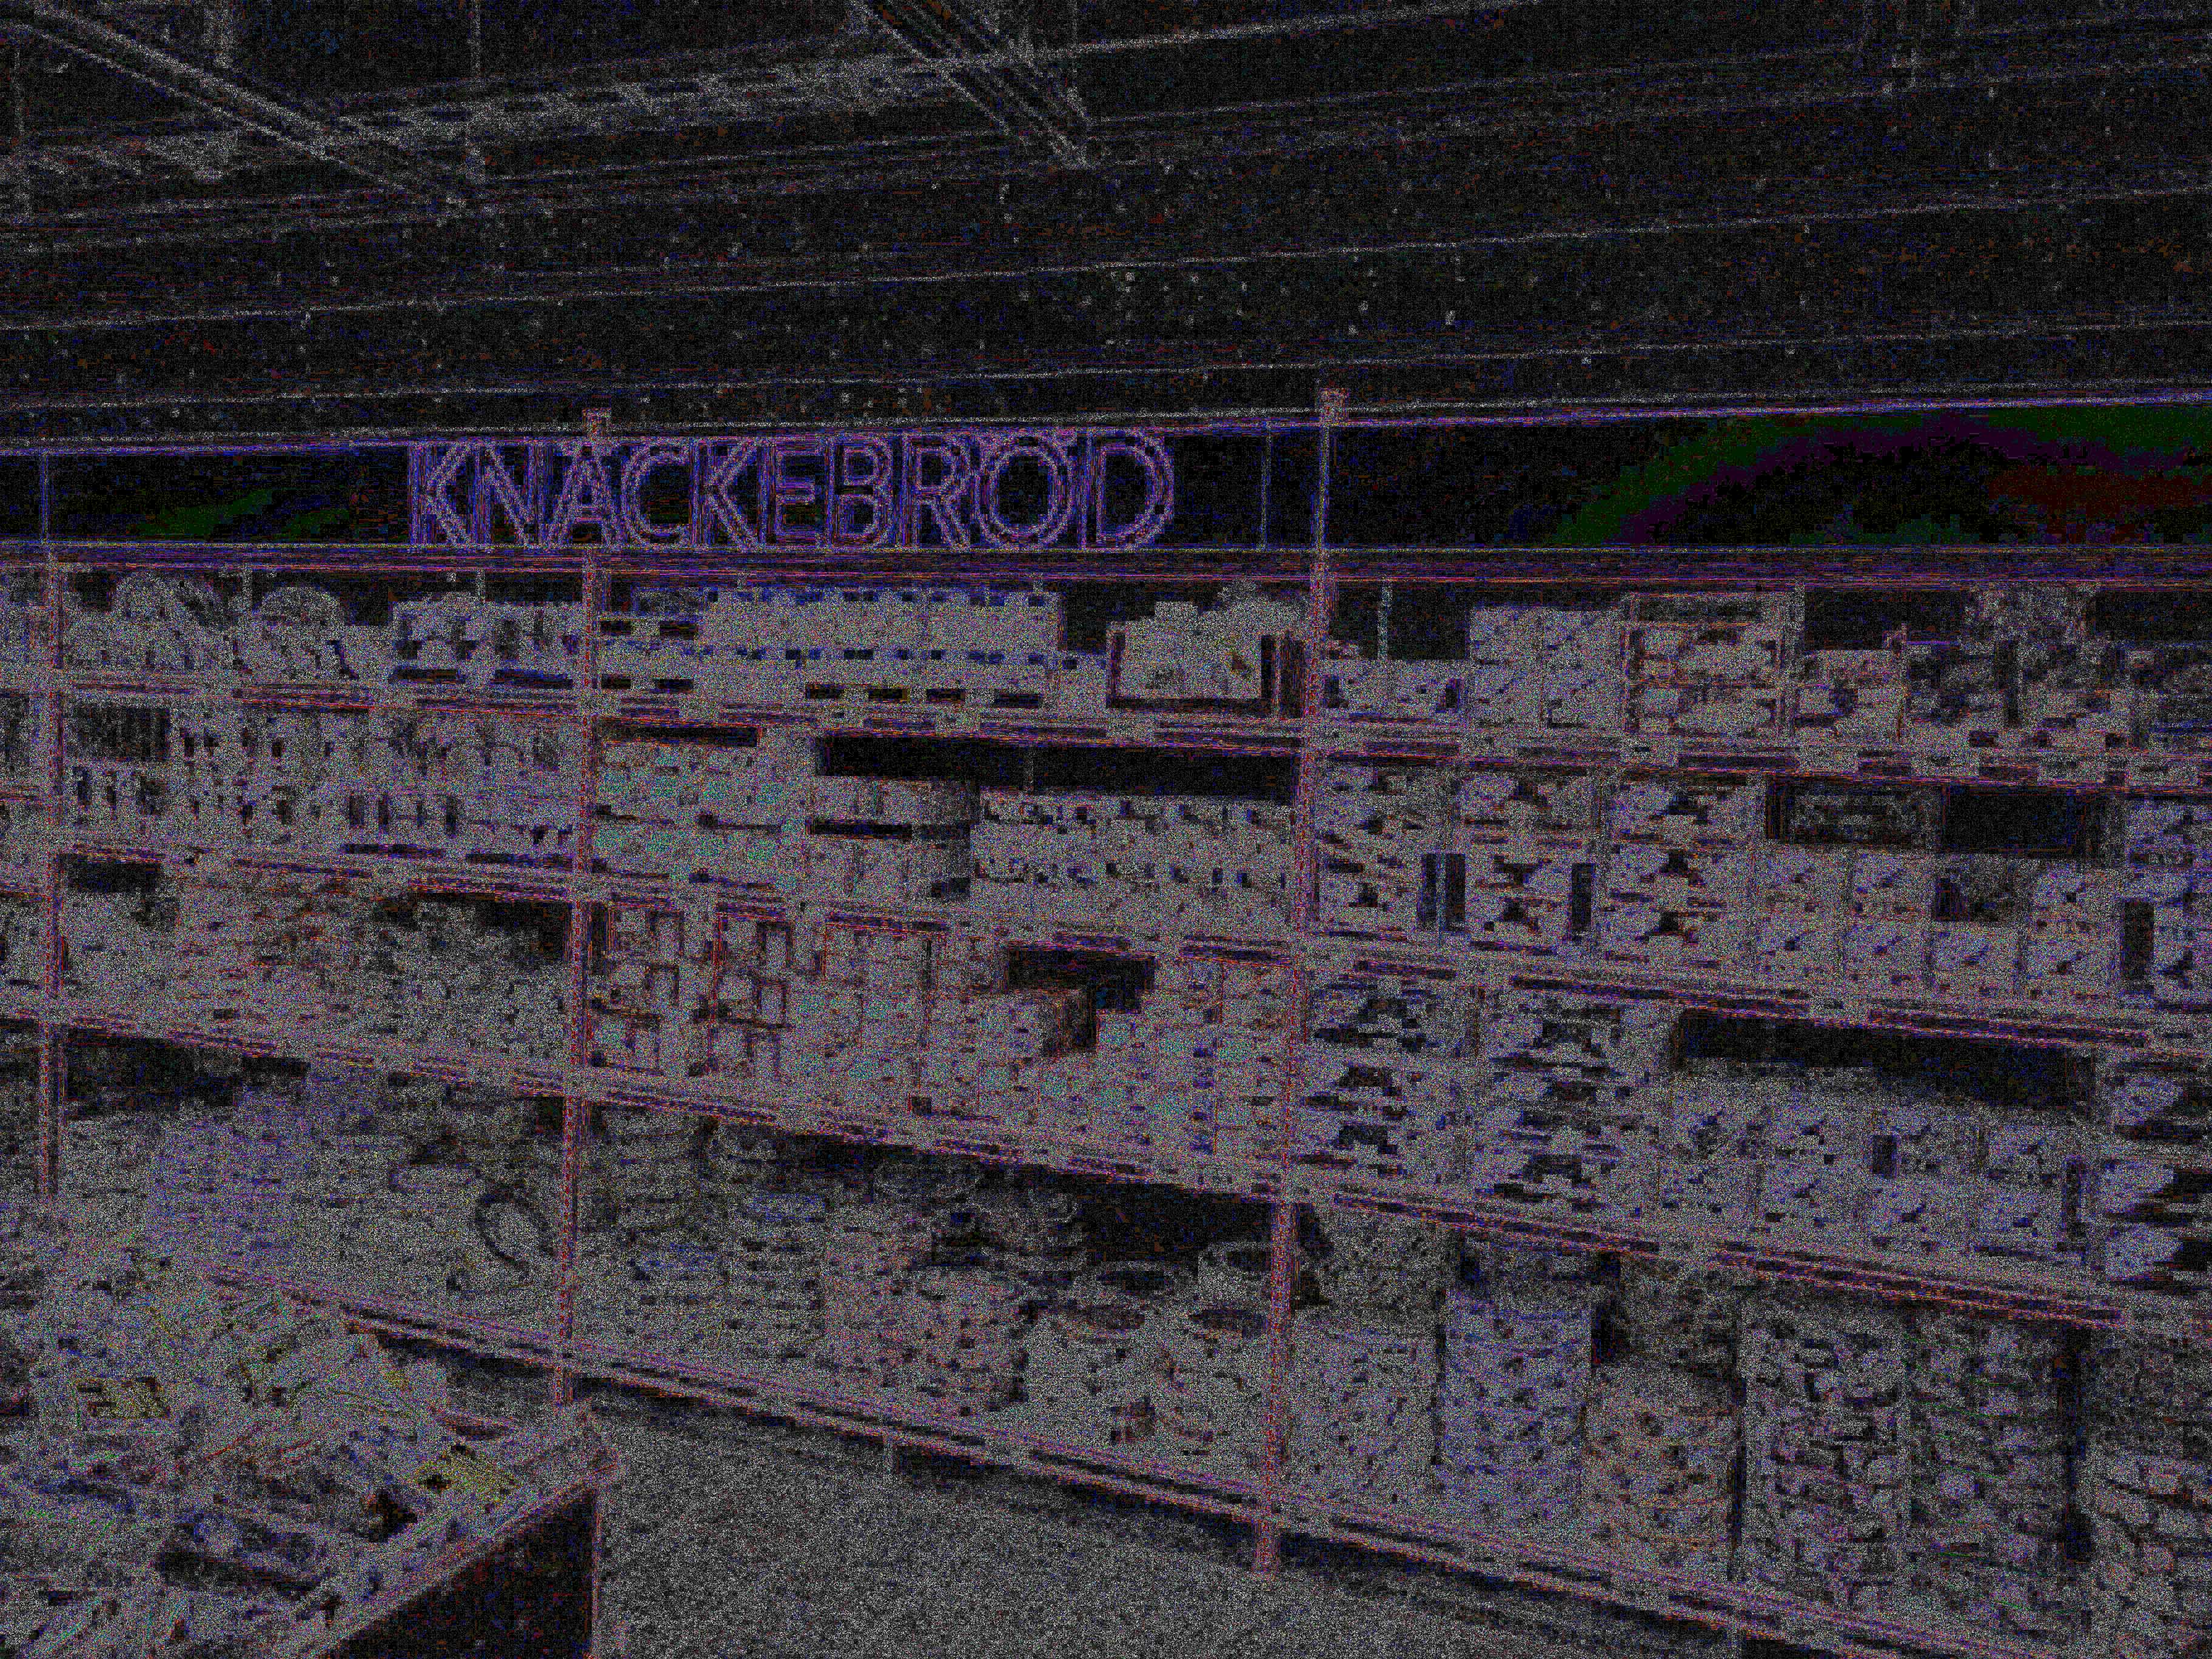
\includegraphics[width=0.4\linewidth]{images/knackebrot/originalELA.jpg}
		\caption{ELA mit Originalbild}
		\label{fig:elaOriginal}
	\end{center}
\end{figure}
\begin{figure}[H]
	\begin{center}
		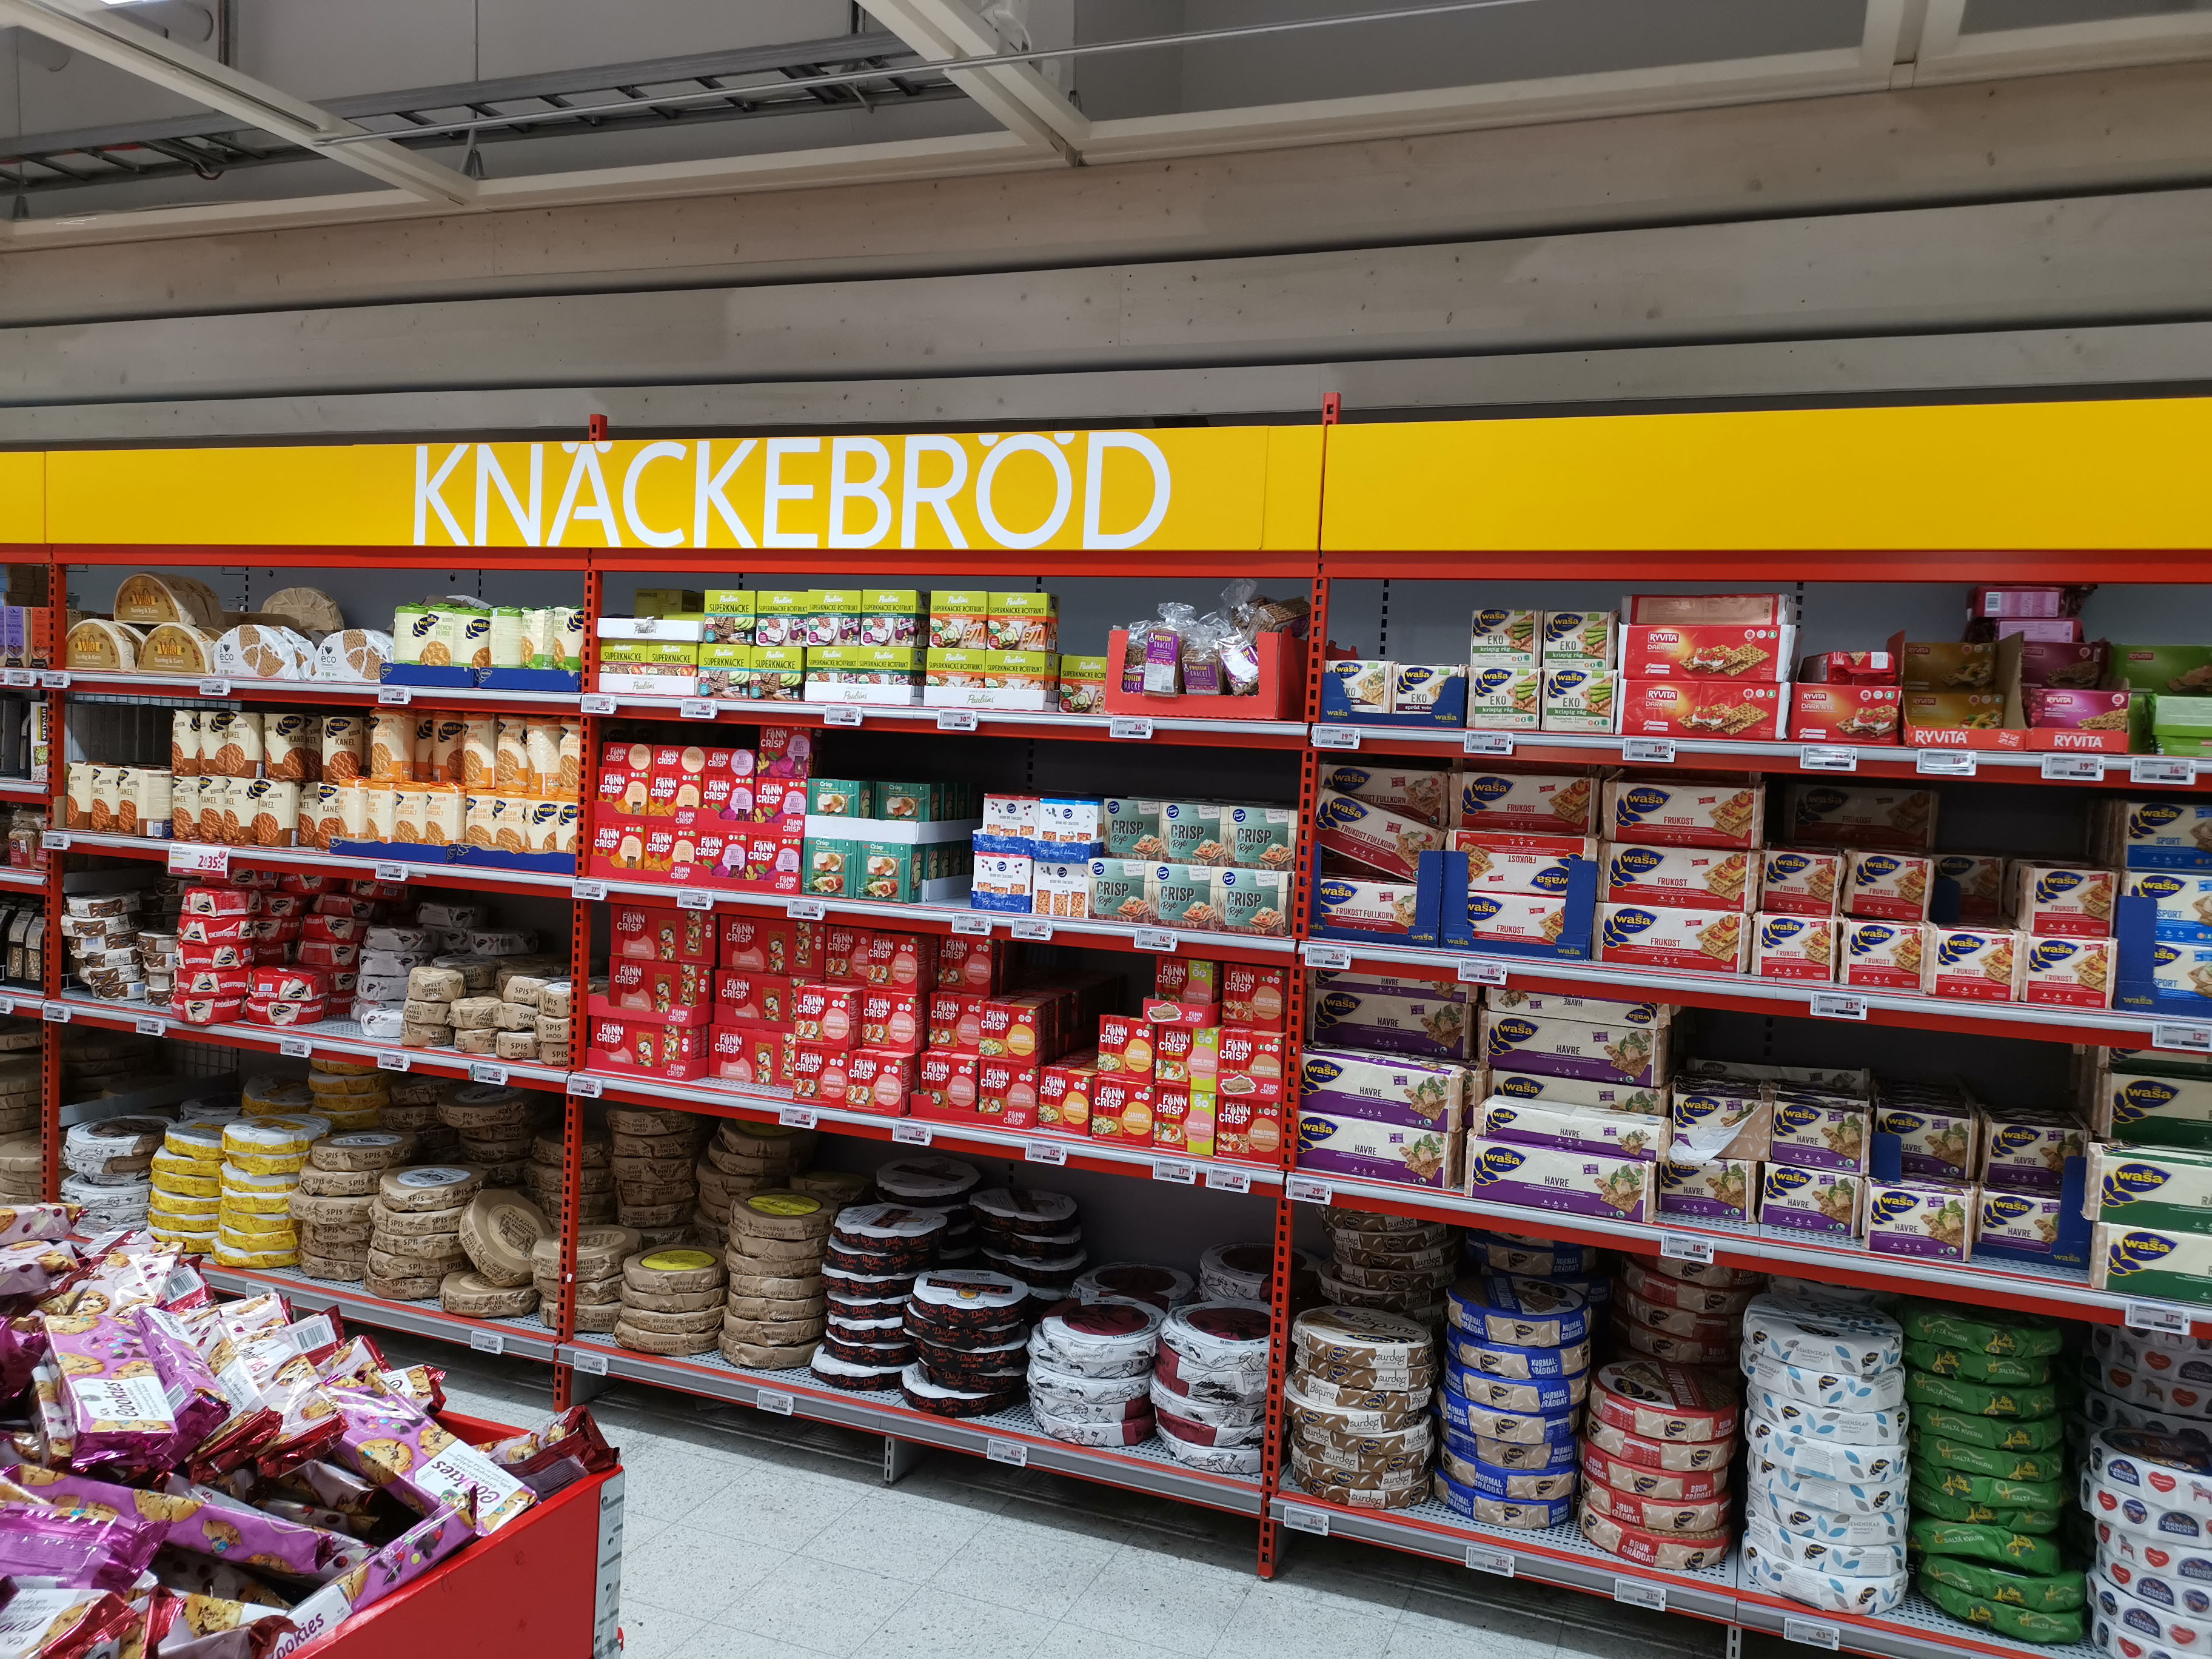
\includegraphics[width=0.4\linewidth]{images/knackebrot/photoshopQualityLevel8.jpg}
		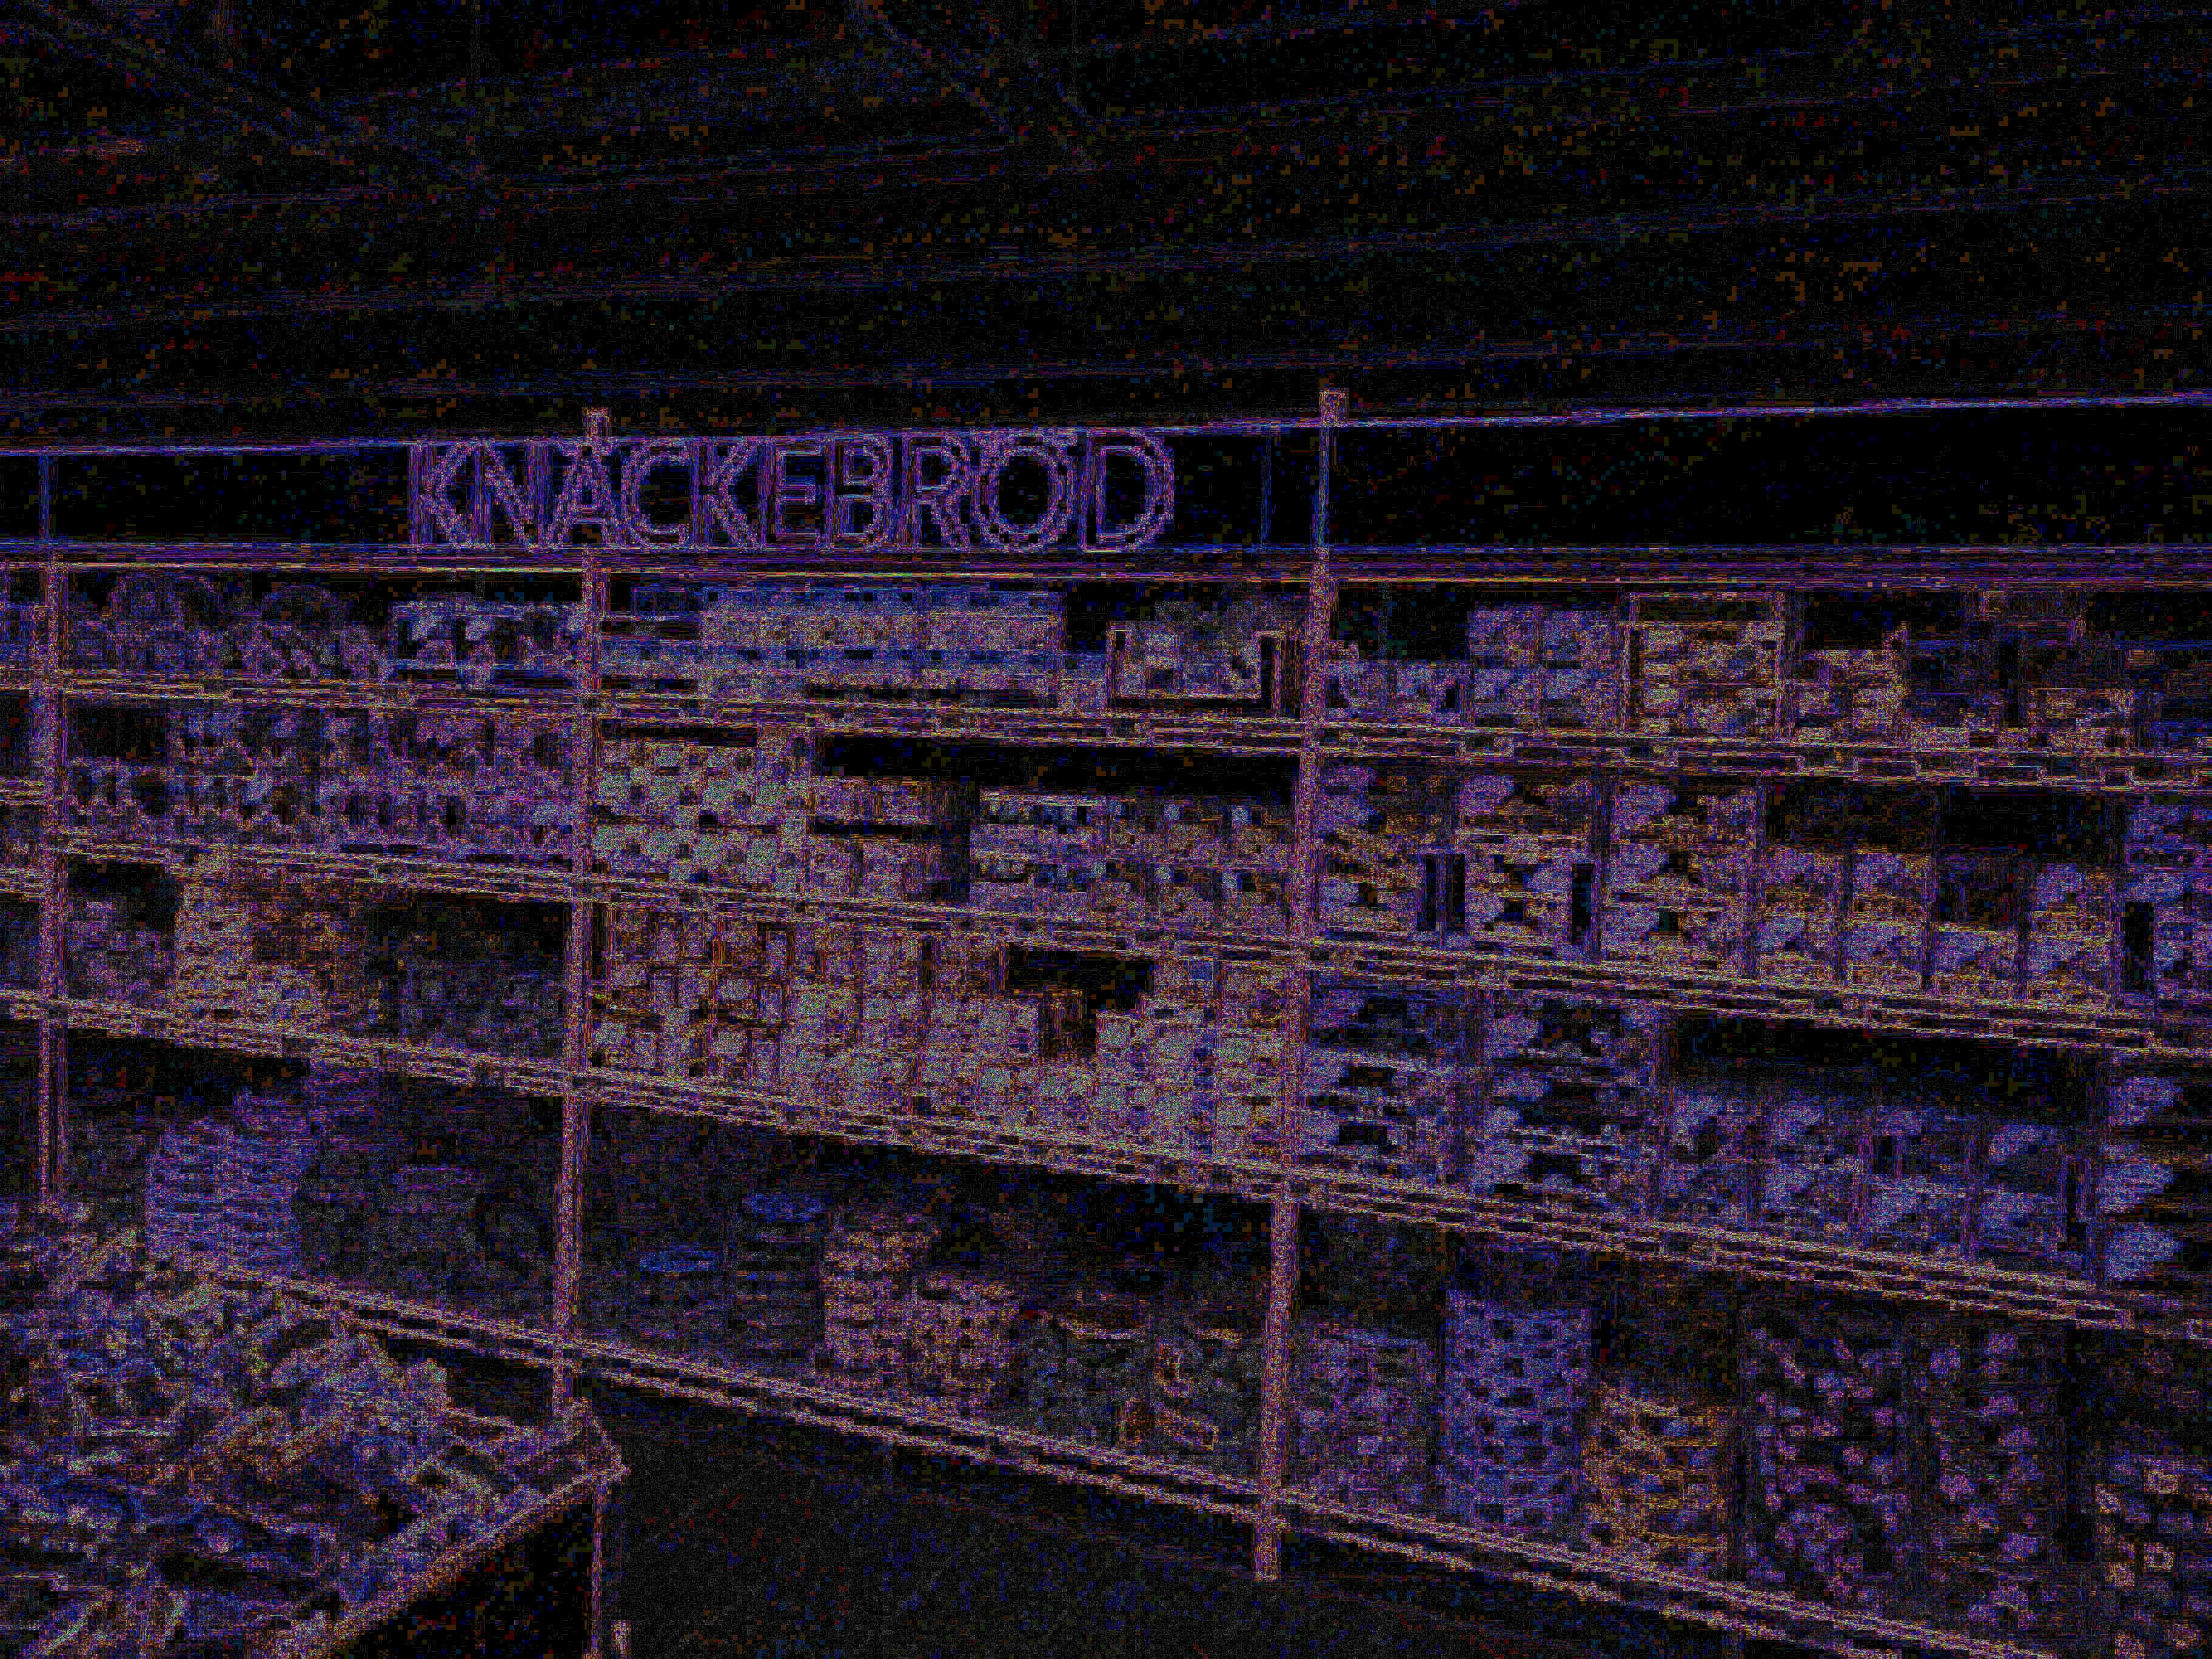
\includegraphics[width=0.4\linewidth]{images/knackebrot/photoshopQualityLevel8ELA.jpg}
		\caption{ELA nach speichern mit Adobe Photoshop 70\%}
		\label{fig:elaPhotoshop}
	\end{center}
\end{figure}
\begin{figure}[H]
	\begin{center}
		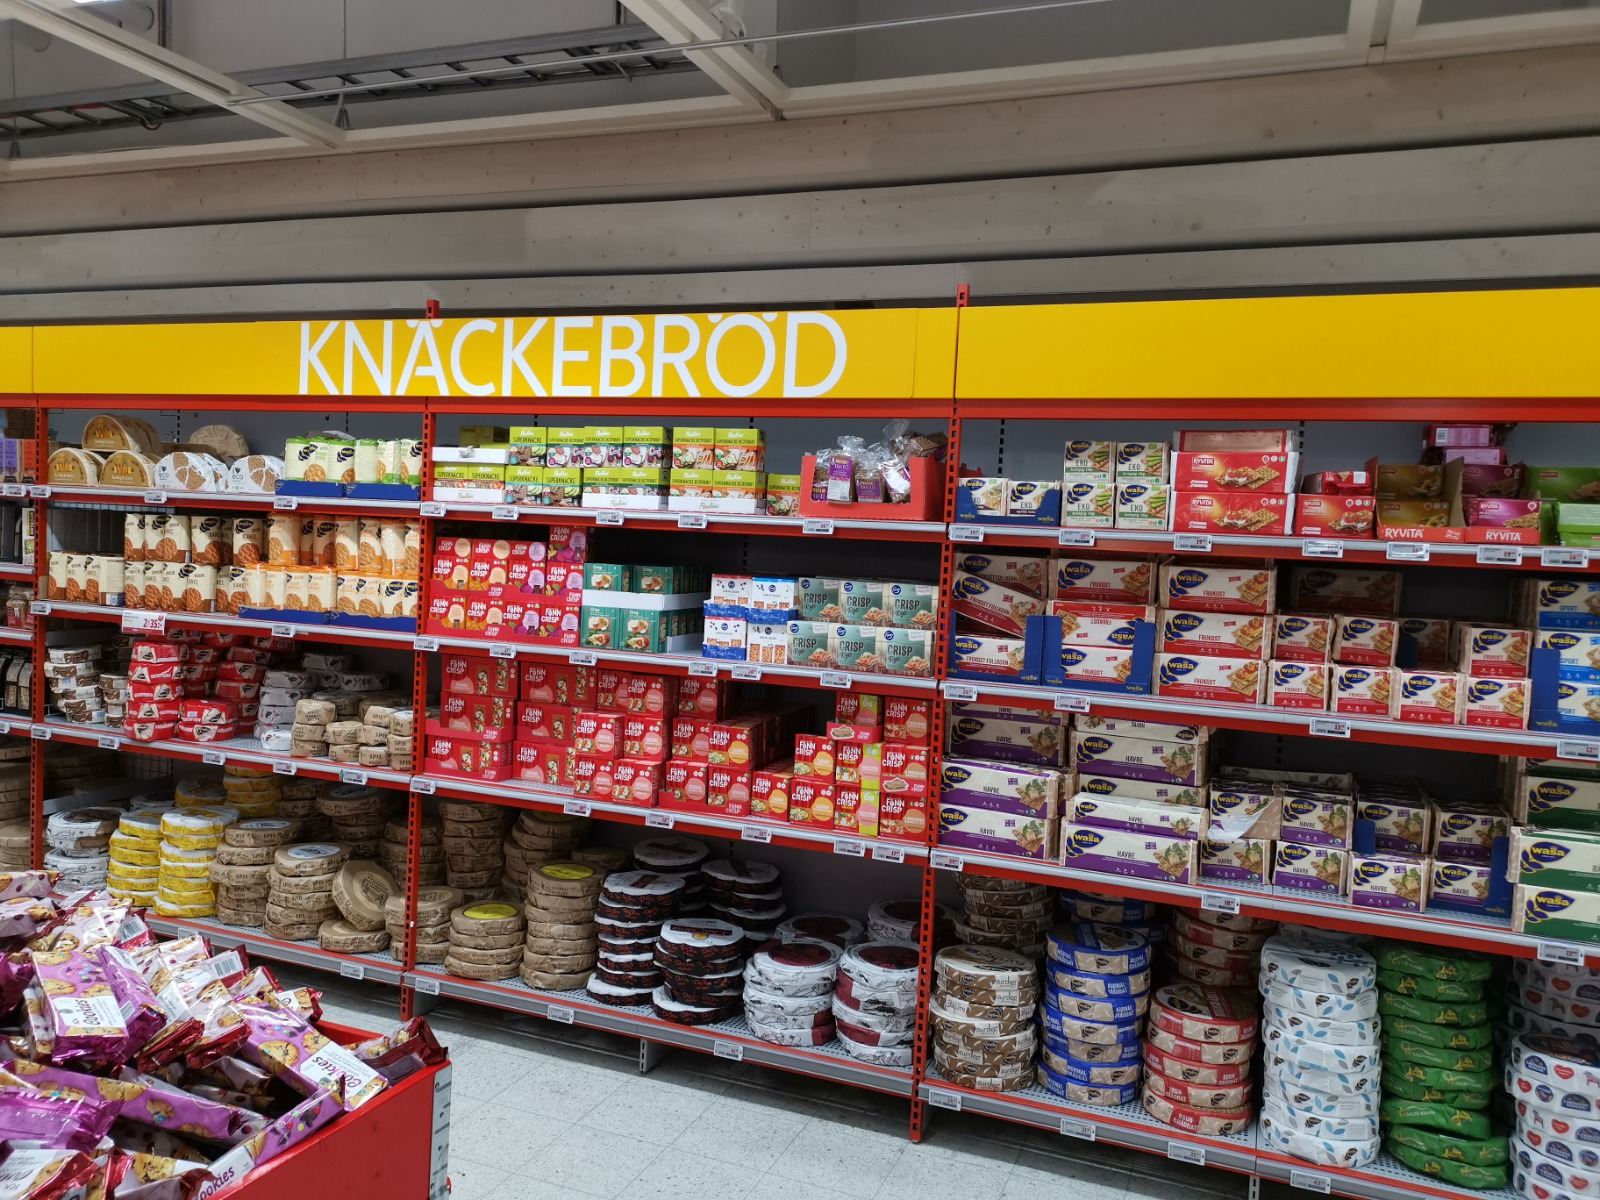
\includegraphics[width=0.4\linewidth]{images/knackebrot/whatsapp.jpg}
		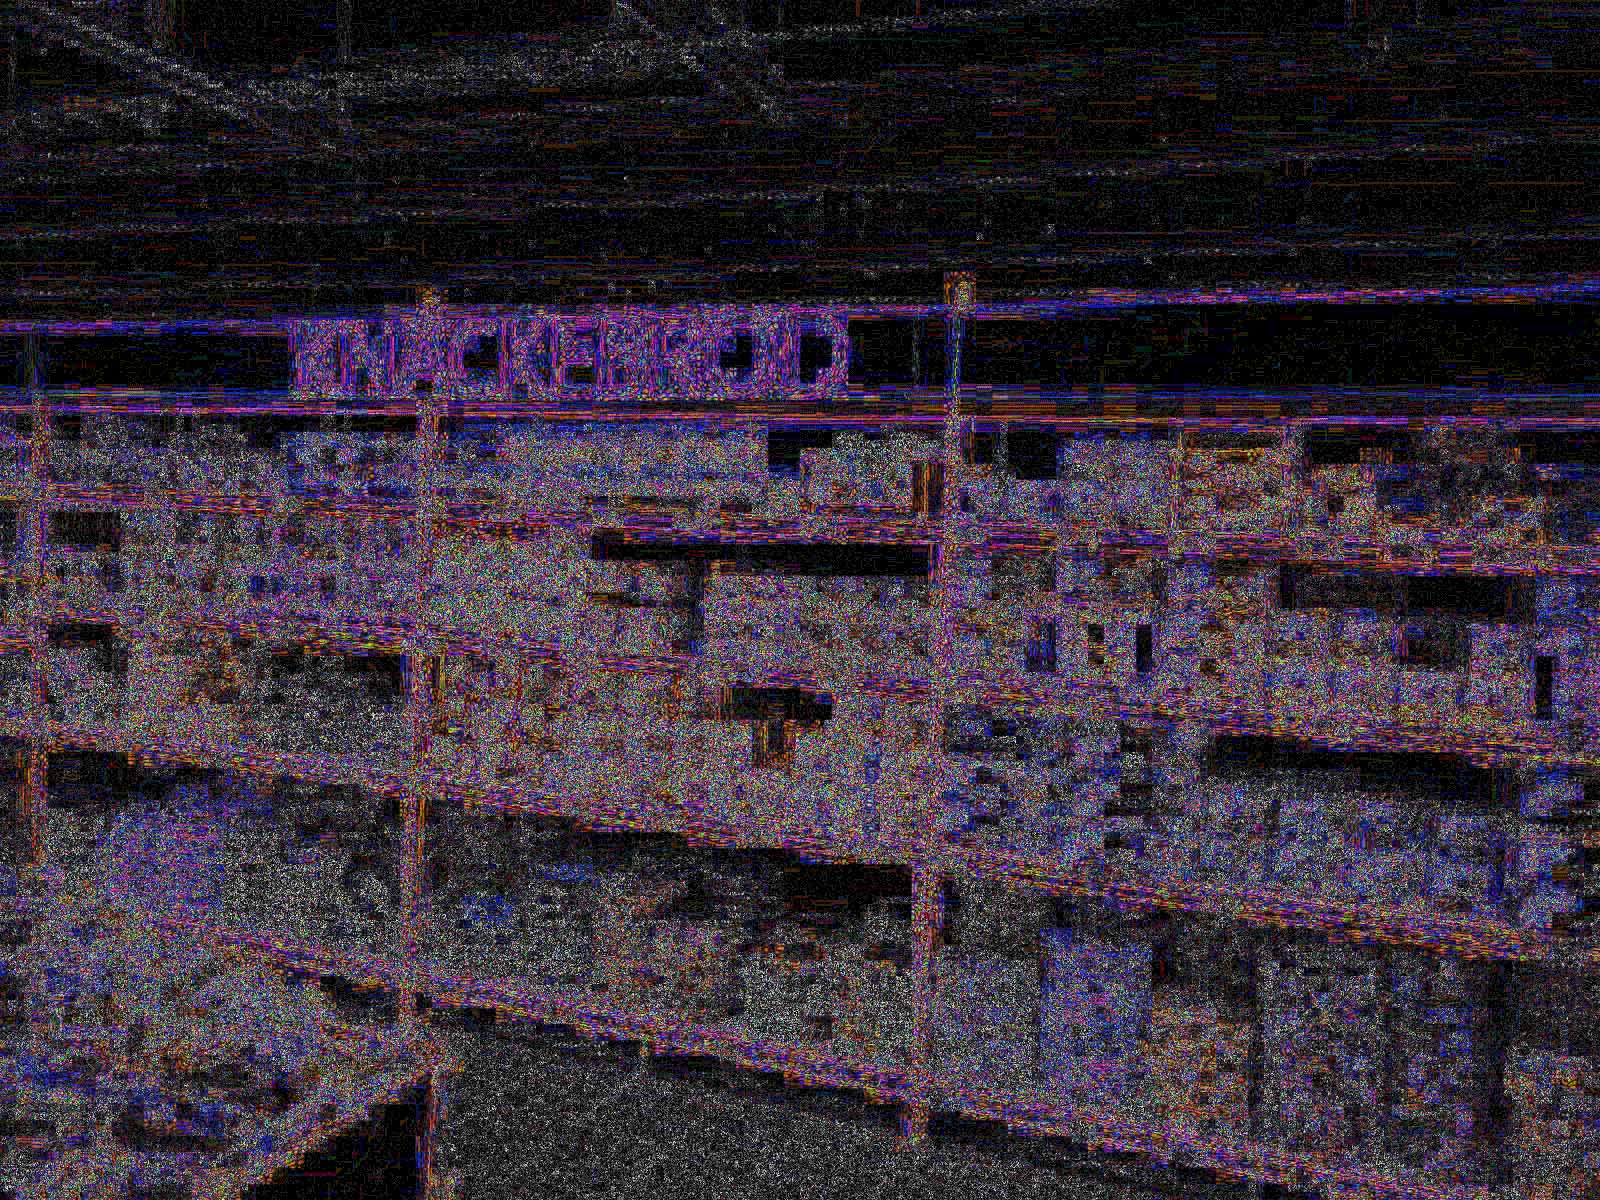
\includegraphics[width=0.4\linewidth]{images/knackebrot/whatsappELA.jpg}
		\caption{ELA nach versendet über Whatsapp}
		\label{fig:elaWhatsapp}
	\end{center}
\end{figure}

\autoref{fig:elaWhatsapp} zeigt das Bild welches in Adobe Photoshop komprimiert wurde und nachdem es über den Messenger Whatsapp versendet wurde. Bei diesem Schritt wurde zudem die Auflösung deutlich reduziert, was die Ursache dafür ist, dass es wieder heller im Vergleich zu dem Bild aus Adobe Photoshop ist. Durch die Änderung der Auflösung weisen die Bereiche welche vorher schon nahe an ihrem lokalen Fehlerminimum waren, also die dunklen, wieder eine große Menge an Veränderungen auf und erscheinen somit heller als im Schritt zuvor.

\section{Bildmanipulation}
Mit dem in \autoref{chap:mehrfachkompression} gewonnenen Erkenntnissen ist es nun möglich in einem generierten ELA-Bild Hinweise auf eine Bildmanipulation zu finden. Das Originalbild ist wieder in \autoref{fig:elaOriginal2} zu sehen und \autoref{fig:elafake} zeigt dieses mal eine Bildmontage bei welche an der linken Seite Knäckebrot durch Toilettenpapier ersetzt wurde, auf der rechten Seite Knäckebrot durch Seife ersetzt und über dem Regal noch ein Krümelmonster eingefügt wurde.\\
betrachtet man die Bildmanipulation für sich fällt dem Betrachter in den meisten Fällen vermutlich des Krümelmonster auf welches offensichtlich nicht echt ist. Bei genauerer Betrachtung fällt dann auch auf, dass Toilettenpapier und Seife auch nicht in das Bild passen.\\
Betrachtet man aber nur die Ausgabe der ELA, ist der erste Bildteil welcher ins Auge fällt der Teil mit dem Toilettenpapier, da dieser deutlich dunkler dargestellt wird als andere Teile des Regals. Das hat die Ursache, dass das eingefügte Bild vermutlich schon mehrfach komprimiert und abgespeichert wurde und es sich somit schon nahe am lokalen Kompressionsminimum befindet. Im mittlerer unveränderte Teil des Bildes befinden sich noch die Pixel vom Originalbild welche sich weit entfernt von ihrem lokalen Kompressionsminimum befinden. So kommt der hohe Kontrast zwischen diesen Bereich zustande welcher ein definitiver Hinweis darauf ist, dass es sich hier um eine Bildmontage handelt.

\begin{figure}[H]
	\begin{center}
		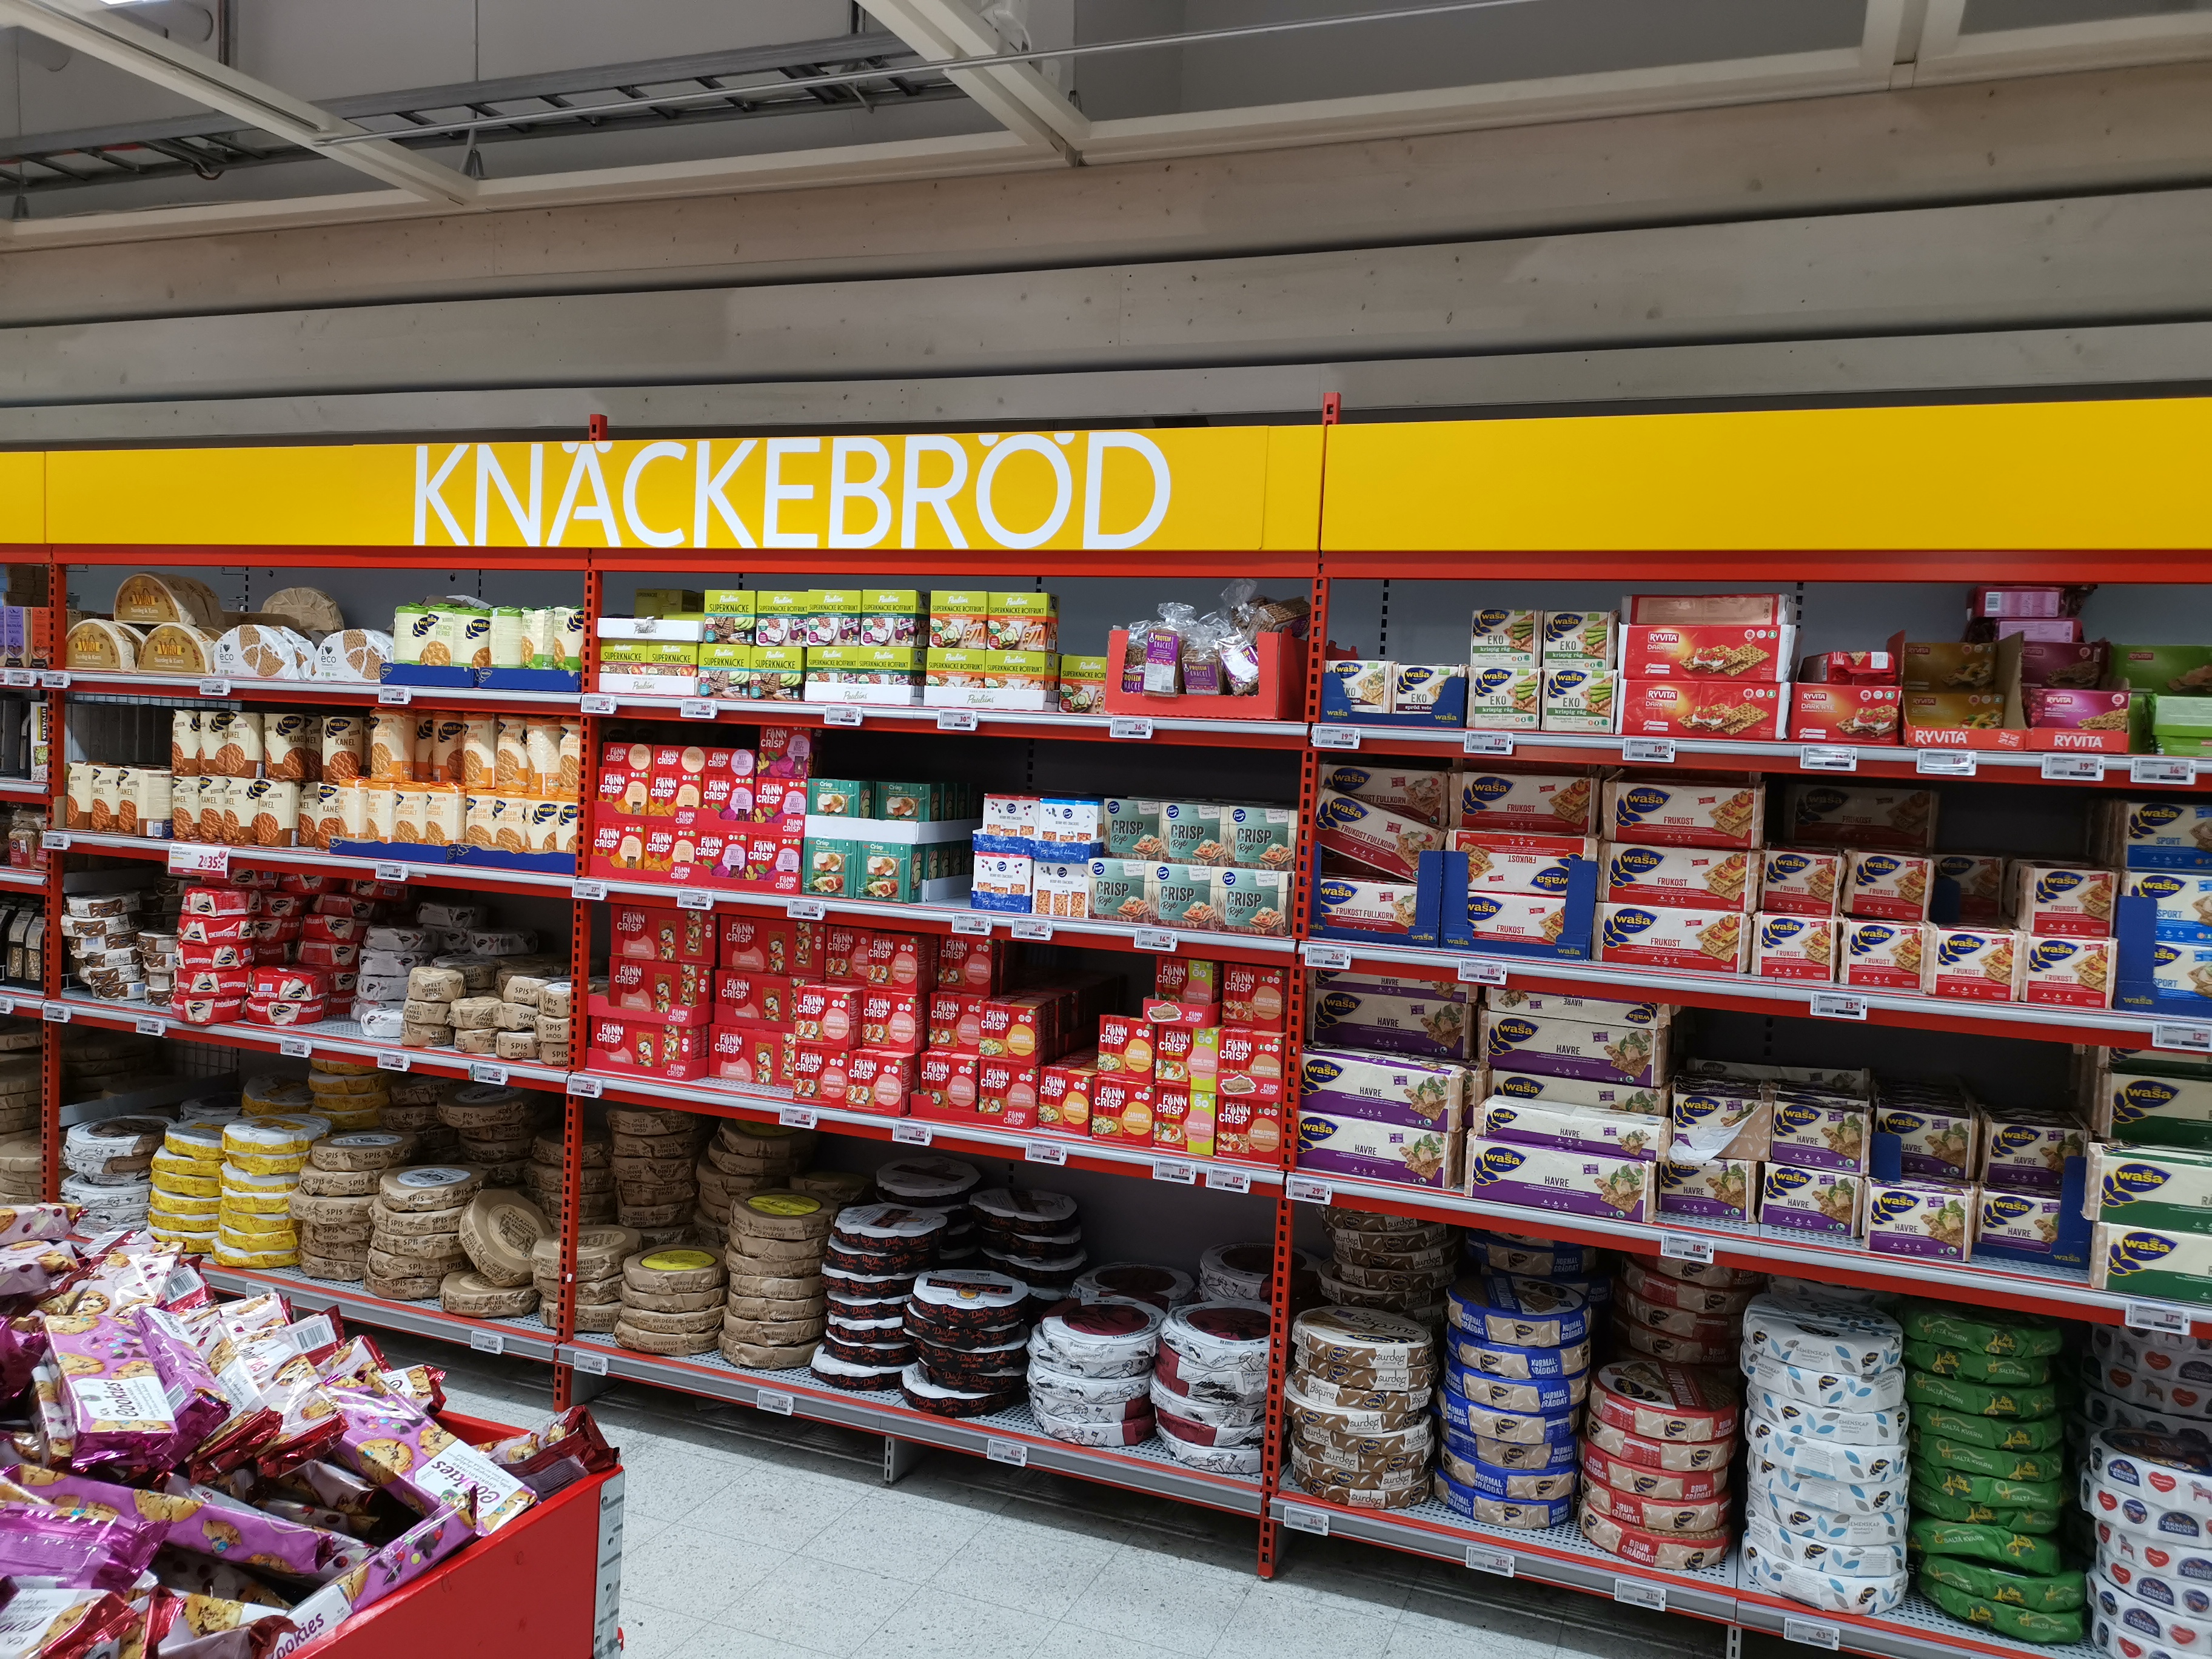
\includegraphics[width=0.4\linewidth]{images/knackebrot/original.jpg}
		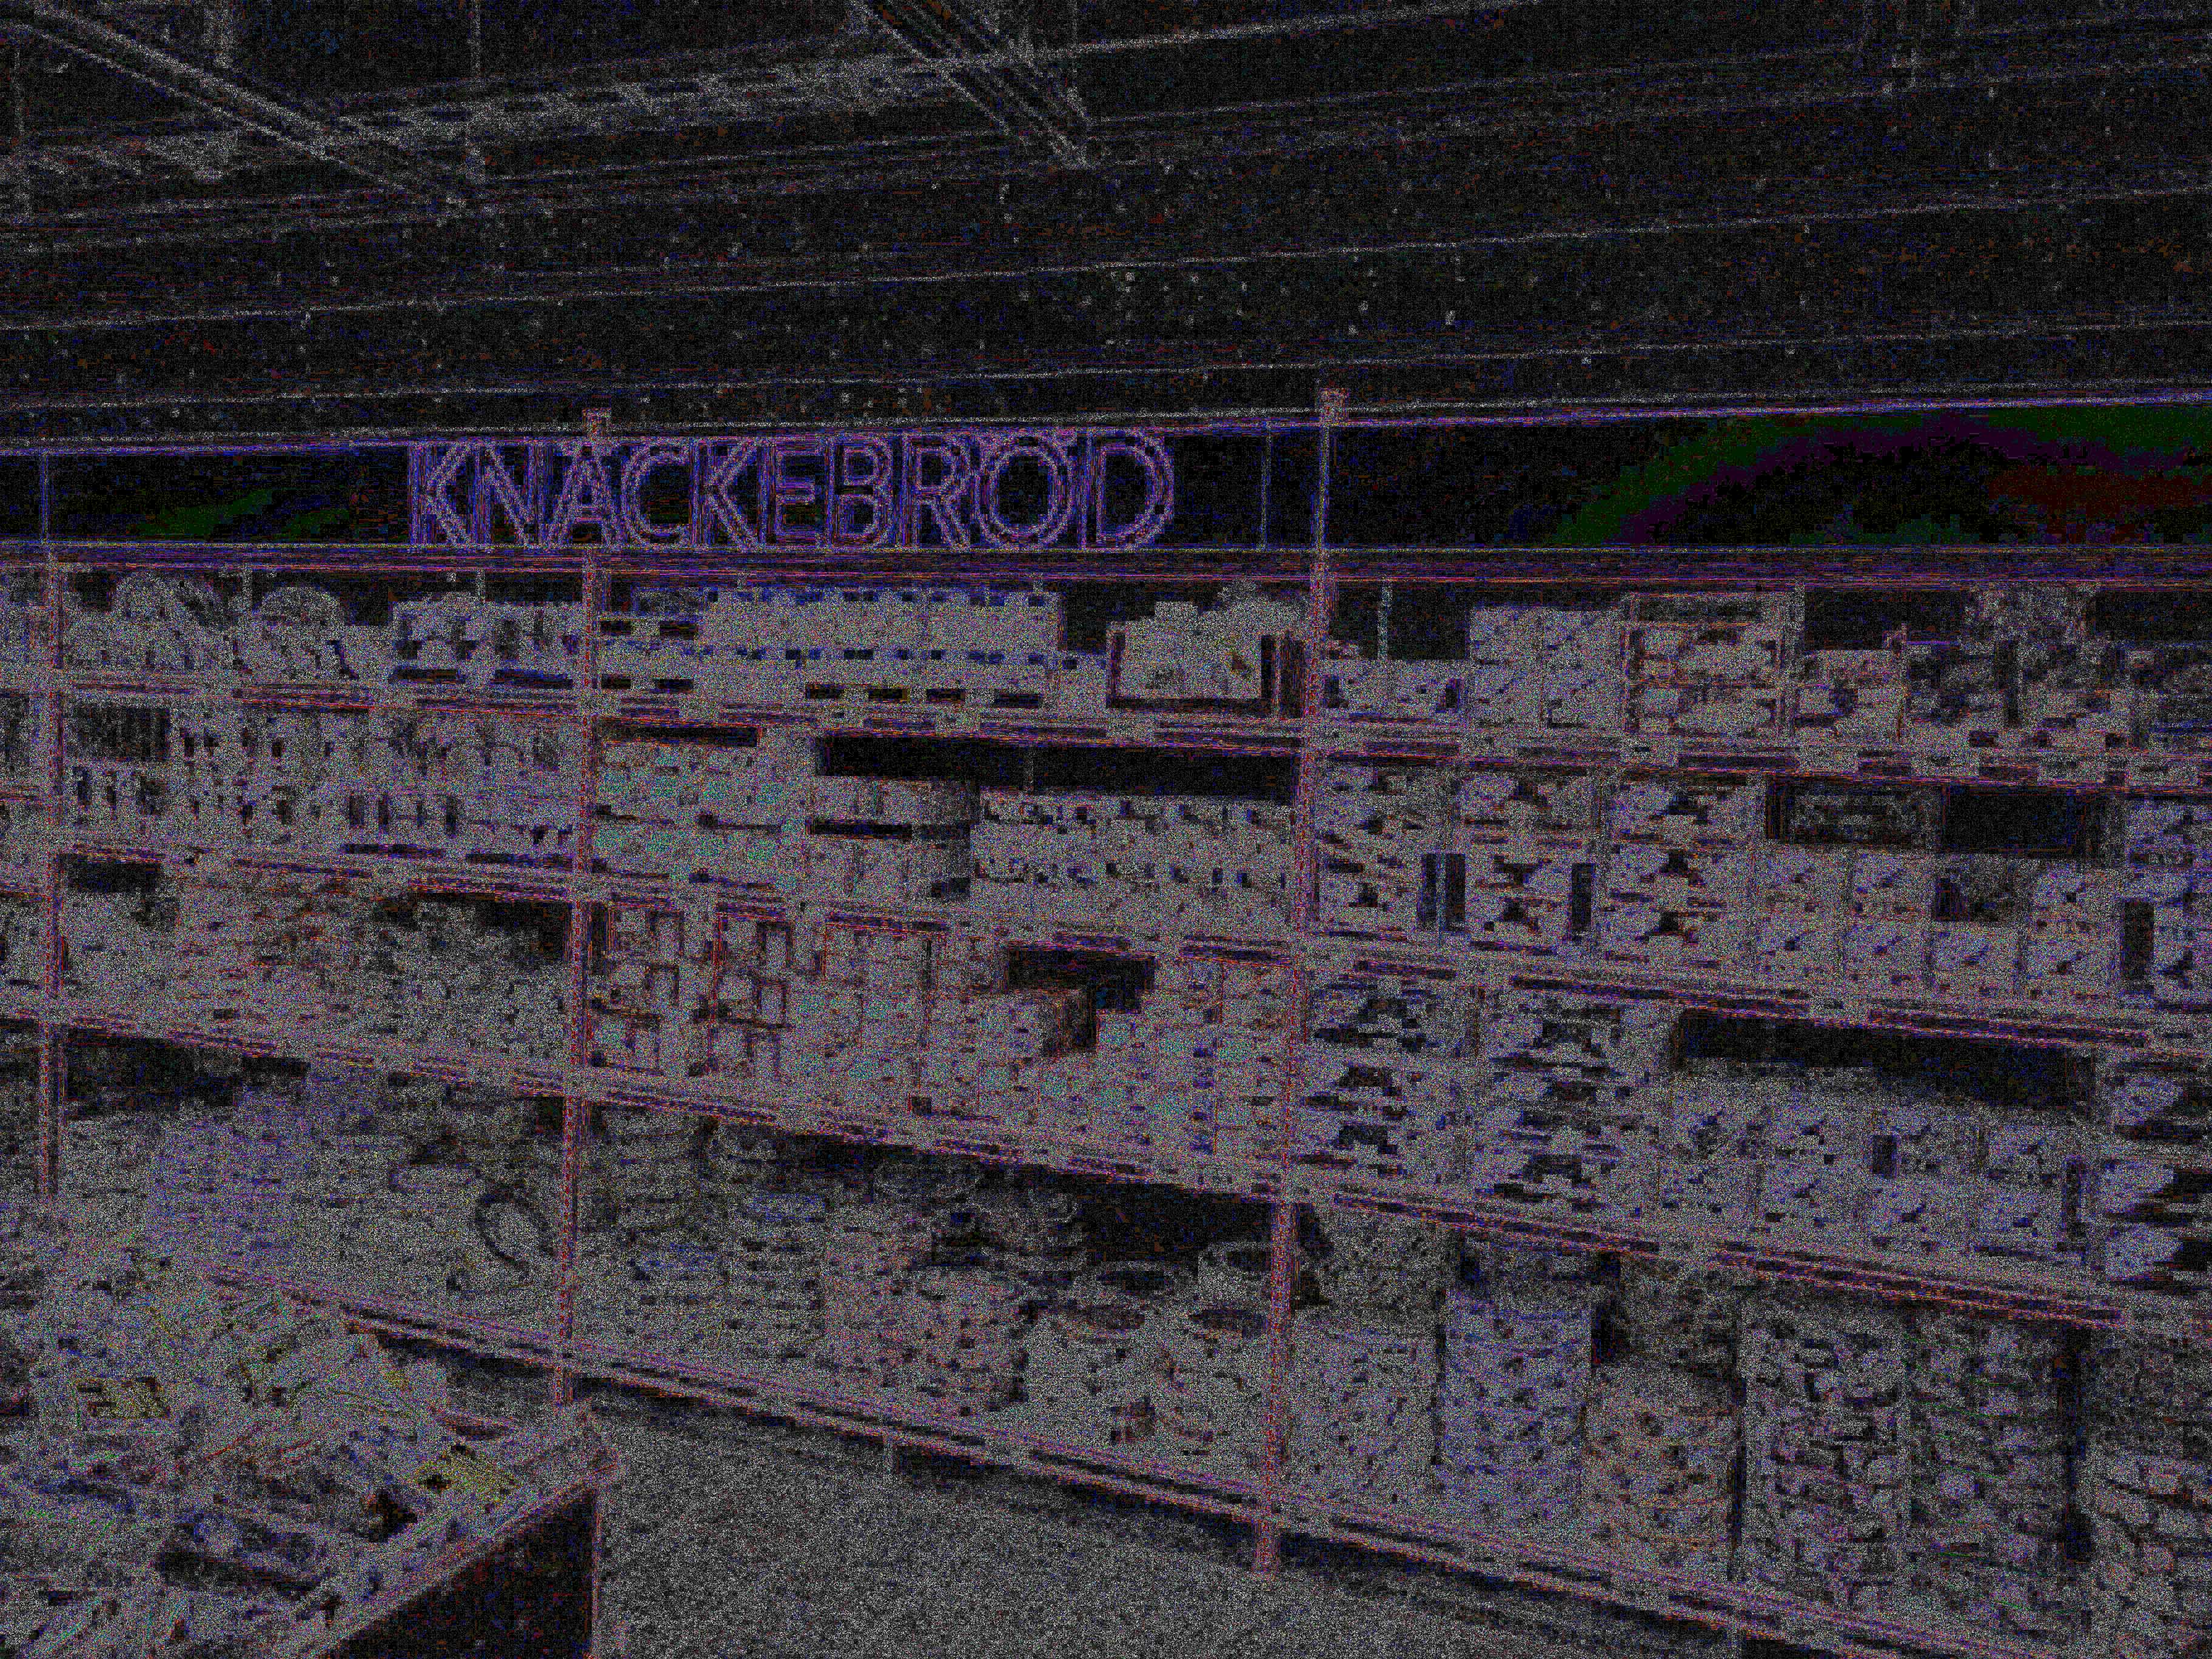
\includegraphics[width=0.4\linewidth]{images/knackebrot/originalELA.jpg}
		\caption{ELA mit Originalbild}
		\label{fig:elaOriginal2}
	\end{center}
\end{figure}
\begin{figure}[H]
	\begin{center}
		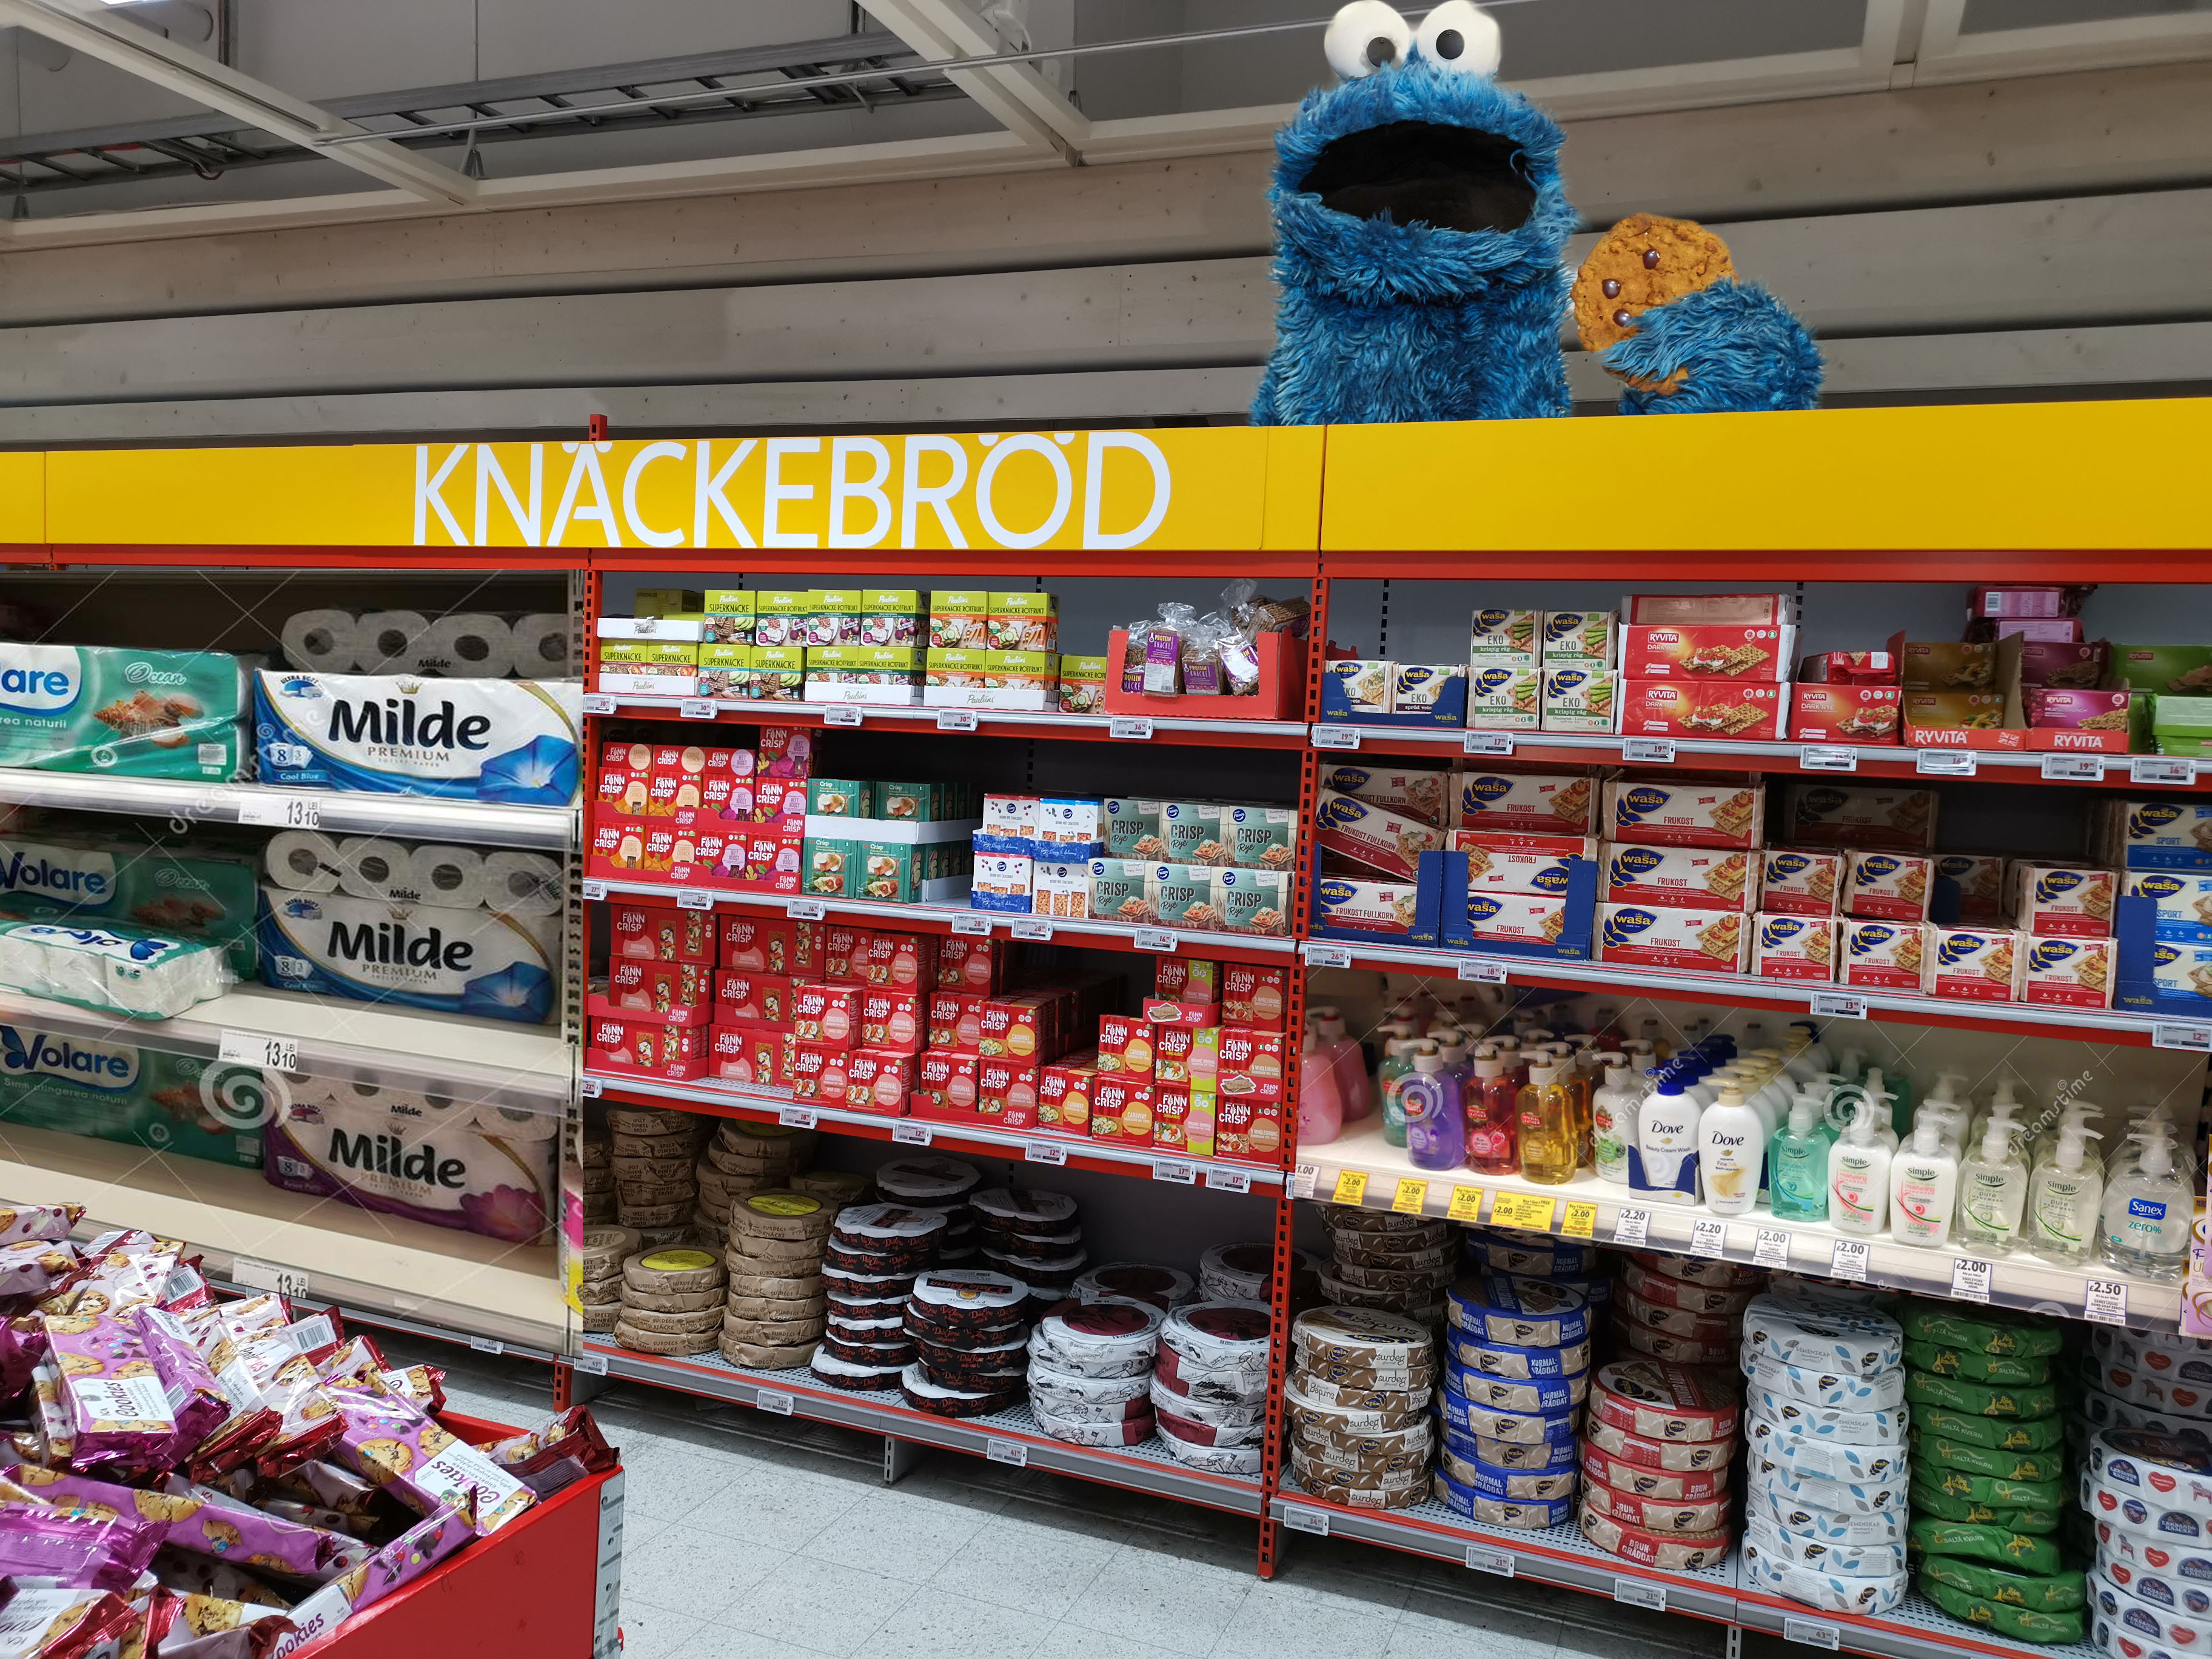
\includegraphics[width=0.4\linewidth]{images/knackebrot/fake.jpg}
		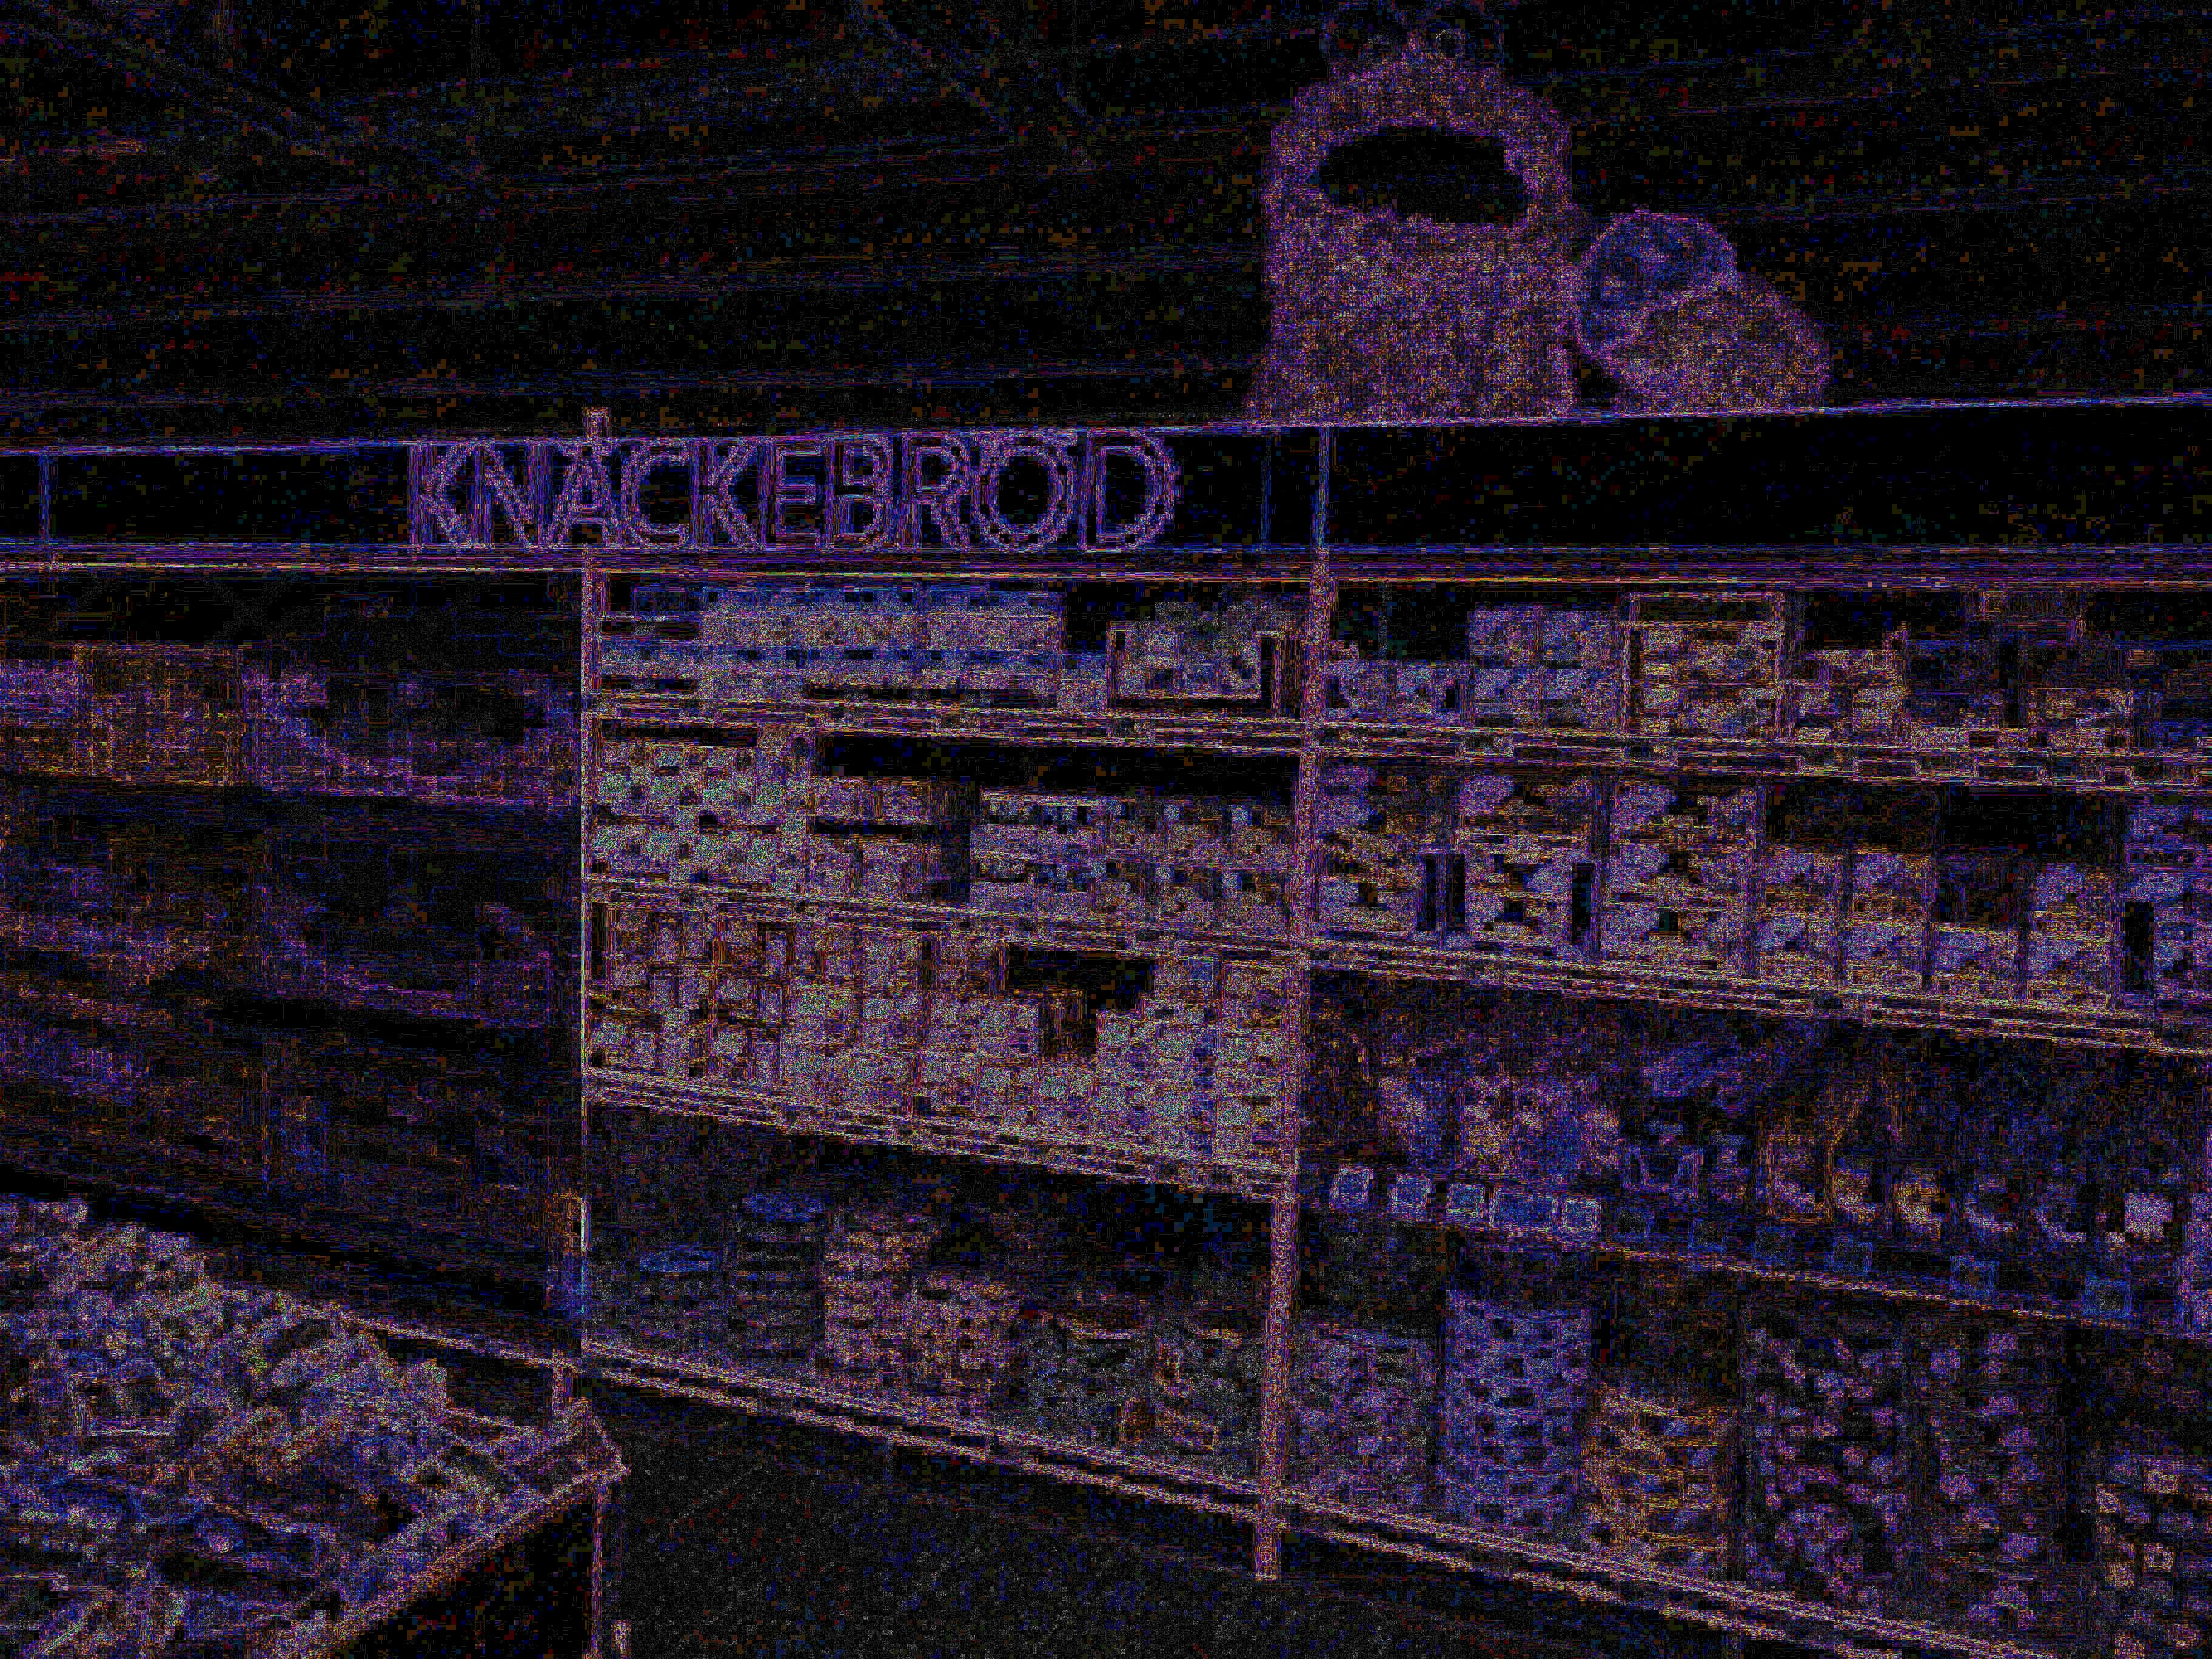
\includegraphics[width=0.4\linewidth]{images/knackebrot/fakeELA.jpg}
		\caption{Bildmontage}
		\label{fig:elafake}
	\end{center}
\end{figure}

\chapter{Zusammenfassung}
dtzjtukjztukzukzukuk










